{{服务\textbf{指下层为相邻上层提供的功能调用}}{。}}协议是水平的,而服务则是垂直的,即下层向上层通过接口提供服务。服务分为以下3类:

\textbf{{1. 面向连接}{的服务和面向无连接的服务}}\\

{{\textbf{面向连接的服务}}\textbf{{:}}}当通信双方通信时,要事先建立一条通信线路,该线路包括建立连接、使用连接和释放连接3个过程。TCP协议就是一种面向连接服务的协议,电话系统就是一个面向连接的模式。\\
{\textbf{面向无连接的服务:}}通信双方不需要事先建立一条通信线路,而是把每个带有目的地址的包(报文分组)传送到线路上,由系统选定路线进行传输。IP协议和UDP协议就是两种无连接服务的协议,邮政系统就是一个无连接的模式。\\
面向连接与面向无连接的对比见表1-1。

~~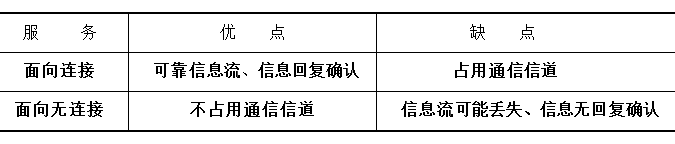
\includegraphics[width=3.46875in,height=0.73958in]{png-jpeg-pics/A29E1A87A8661A89CCCAC4686C76F18A.png}

\textbf{{2. 有应答服务与无应答服务}}\\

\textbf{有应答服务:}指接收方在收到数据后向发送方给出相应的应答。\\
\textbf{无应答服务:}指接收方收到数据后不自动给出应答。

\textbf{{3. 可靠服务与不可靠服务}}

{\textbf{可靠服务:}}指网络具有检错、纠错、应答机制,能保证数据正确、可靠地传送到目的地。\\
{\textbf{不可靠服务:}}指网络不能保证数据正确、可靠地传送到目的地,网络只能是尽量正确、可靠,是一种``尽力而为''的服务。\\

{\textbf{{注意:}}并非在一个层内完成的全部功能都称为服务,只有那些能够被高一层实体``看得见''的功能才称为服务。}
